\documentclass[12pt]{article}
\usepackage{seantex}
\usepackage{pgfplots}

% --- Document Info ---
\title{Analysis II: Serie 10}
\author{Sean Findlay}
\date{\today}

% --- Start Document ---
\begin{document}

\maketitle

\begin{problem}{Spherical quadrilateral}{}
    Calculate the area of the spherical quadrilateral $S \subset \mathbb{S}^2$ bounded by the meridians $-\pi < \phi_1 < \phi_2 < \pi$ and parallels $-\frac{\pi}{2} < \theta_1 < \theta_2 < \frac{\pi}{2}$
\end{problem}

Apply the change of variables $\psi$ given by the following map (spherical coordinates with radius $r = 1$, we need $\theta = 0$ to give us $z = 0$):
\begin{align*}
    \begin{pmatrix} \phi \\ \theta \end{pmatrix} \mapsto \begin{pmatrix} x \\ y \\ z \end{pmatrix} := \begin{pmatrix} \cos\theta \cos\phi \\ \cos\theta\sin\phi \\ \sin\theta \end{pmatrix}
\end{align*}

The Jacobian of $\psi$ is:
\begin{align*}
    J\psi = 
    \begin{pmatrix}
        -\cos\theta\sin\phi & -\sin\theta\cos\phi \\
        \cos\theta\cos\phi & -\sin\theta\sin\phi \\
        0 & \cos\theta
    \end{pmatrix}, \quad J\psi^T = 
    \begin{pmatrix}
        -\cos\theta\sin\phi & \cos\theta\cos\phi & 0 \\
        -\sin\theta\cos\phi & -\sin\theta\sin\phi & \cos\theta \\
    \end{pmatrix}
\end{align*}

So the Gram determinant is
\begin{align*}
    \sqrt{\det(J \psi^T J\psi)} &= \sqrt{\det
    \begin{pmatrix}
        \cos^2\theta\sin^2\phi + \cos^2\theta\cos^2\phi & 0 \\
        0 & \sin^2\theta\cos^2\phi + \sin^2\theta\sin^2\phi + \cos^2\theta \\
    \end{pmatrix}} \\
    &= \sqrt{\det
    \begin{pmatrix}
        \cos^2\theta\ & 0 \\
        0 & 1 \\
    \end{pmatrix}} = \sqrt{\cos^2\theta} = \cos\theta
\end{align*}

Thus, the area is given by: 
\begin{align*}
    \int_\R \int_\R \mathds{1}_S \dd y \dd x &= \int_{\phi_1}^{\phi_2} \int_{\theta_1}^{\theta_2} \cos\theta \dd \theta \dd \phi = \int_{\phi_1}^{\phi_2} \dd \phi \int_{\theta_1}^{\theta_2} \cos\theta \dd \theta \\
    &= (\phi_2 - \phi_1) \cdot \big[ \sin\theta \big]_{\theta_1}^{\theta_2} = \boxed{(\phi_2 - \phi_1) \cdot (\sin\theta_2 - \sin\theta_1)}
\end{align*}

\newpage

\begin{problem}{Surface area of a torus}{}
    Let $S = \{(x, y, 0) \in \R^3 \ |\ x^2 + y^2 = 4\}$ and $T = \{x \in \R^3\ |\ d_S(x) \leq 1\}$, where $d_S = \inf\{|x-y| \ |\ y \in S\}$ denotes the minimal distance from $S$ to $x \in R^3$. Parametrise $\partial T$ and then calculate the area.
\end{problem}

We can parametrise the points on $S$ first with $\vphi \in [0, 2\pi]$. Define a map $\Phi: [0, 2\pi] \rightarrow S$:
\begin{align*}
    \Phi(\vphi) = \begin{pmatrix} x \\ y \\ 0 \end{pmatrix} = \begin{pmatrix} 2\sin\vphi \\ 2\cos\vphi \\ 0 \end{pmatrix}
\end{align*}

Next, for all points in $S$, parametrise the points with $d_S \leq 1$ using $\theta \in [0, 2\pi]$. Define a map $\Psi: [0, 2\pi] \times [0, 2\pi] \rightarrow \partial T$:
\begin{align*}
    \Psi(\vphi, \theta) = \underbrace{\Phi(\vphi)}_{\text{point on } S} + \underbrace{\nu_{\vphi} \cos\theta}_{\text{direction normal to } S} + \underbrace{\begin{pmatrix} 0 \\ 0 \\ 1 \end{pmatrix} \sin\theta}_{\text{vertical direction}}
\end{align*}

where $\nu_\vphi$ is the normal vector to the point $\Phi(\vphi)$. Let this normal vector be
\begin{align*}
    \nu_\vphi = \begin{pmatrix} \sin\vphi \\ \cos\vphi \\ 0 \end{pmatrix}
\end{align*}

So we have the following parametrisation of $\partial T$:
\begin{align*}
    \Psi(\vphi, \theta) &= \begin{pmatrix} 2\sin\vphi \\ 2\cos\vphi \\ 0 \end{pmatrix} + \begin{pmatrix} \sin\vphi\cos\theta \\ \cos\vphi\cos\theta \\ 0 \end{pmatrix} + \begin{pmatrix} 0 \\ 0 \\ \sin\theta \end{pmatrix} = (2 + \cos\theta) \begin{pmatrix} \sin\vphi \\ \cos\vphi \\ 0 \end{pmatrix} + \begin{pmatrix} 0 \\ 0 \\ \sin\theta \end{pmatrix}
\end{align*}

Compute the Jacobian of this parametrisation:
\begin{align*}
    J \Psi =
    \begin{pmatrix}
        \cos\vphi(2 + \cos\theta) & -\sin\vphi\sin\theta \\
        -\sin\vphi(2 + \cos\theta) & -\cos\vphi\sin\theta \\
        0 & \cos\theta
    \end{pmatrix}
\end{align*}

The Gram determinant is:
\begin{align*}
    \sqrt{\det(J \Psi^T J\Psi)} &= \sqrt{\det
    \begin{pmatrix}
        (2 + \cos\theta)^2 & 0 \\
        0 & 1
    \end{pmatrix}}
    = 2 + \cos\theta
\end{align*}

Now, calculate the area.
\begin{align*}
    \int_{0}^{2\pi} \int_{0}^{2\pi} (2 + \cos\theta) \dd \theta \dd \vphi &= \int_{0}^{2\pi} \dd \vphi \int_{0}^{2\pi} (2 + \cos\theta) \dd \theta \\
    &= 2\pi \left(\int_{0}^{2\pi} 2 \dd \theta\right) +  2\pi \left(\int_{0}^{2\pi} \cos\theta \dd \theta\right) \\
    &= 8\pi^2 + 2\pi \big[ \sin\theta \big]_{0}^{2\pi} = 8\pi^2 + 2\pi \cdot 0 \\
    &= \boxed{8 \pi^2}
\end{align*}

\begin{problem}{Solids of revolution}{}
    Given $f \in C^1((a, b)) \cap C([a, b])$ such that $f \geq 0$, define the rotational body around the $x$-axis
    \begin{align*}
        \Omega := \left\{ (x, y, z) \in \R^3 \ |\ a < x < b,\ \sqrt{y^2 + z^2} < f(x) \right\} \\
        \partial_{\text{side}}\Omega := \left\{ (x, y, z) \in \R^3 \ |\ a < x < b,\ \sqrt{y^2 + z^2} = f(x) \right\}
    \end{align*}

    \begin{enumerate}
        \item Say whether $\Omega,\ \partial_{\text{side}}\Omega$ are open/closed/connected subsets of $\R^3$.
        \item Show that $\mathrm{vol}_3(\Omega) = \pi \int_{a}^{b} f(x)^2 \dd x$
        \item Show that $\mathrm{vol}_2(\partial_{\text{side}}\Omega) = 2\pi\int_{a}^{b} \sqrt{1 + f'(x)^2}f(x) \dd x$
        \item Calculate the volume and surface area of the "improper rotational body" that arises when $f(x) = \frac{1}{x},\ a = 1,\ b = \infty$.
    \end{enumerate}
\end{problem}

\begin{enumerate}
    \item 
    \begin{itemize}
        \item \underline{$\Omega$}: We can define $p(x, y, z) = x$, and $g(x, y, z) = \sqrt{y^2+z^2} - f(x)$, then $\Omega$ is the intersection of the preimages of the open sets
        \begin{align*}
            \Omega = p^{-1}((a, b)) \cap g^{-1}(-\infty, 0)
        \end{align*}

        Because $f$ is continuous, both $p$ and $g$ are continuous. So the preimage of the open intervals under the continuous functions are open. And the intersection of two open intervals is open. So $\Omega$ is open. It is not closed, because it does not contain its boundary.

        It is possible that we have points $\bar{x} \in (a, b)$ where $f(\bar{x}) = 0$. At these points, we require $\sqrt{y^2+z^2} < 0$, which cannot be satisfied. So at these points $\bar{x}$, there are no points in $\Omega$ with this $x$-value. Thus, a point $\bar{x}$ like this splits $\Omega$ into two separate volumes. So $\Omega$ is connected iff $f(x) > 0\ \forall x \in (a, b)$.

        \item \underline{$\partial_{\text{side}}\Omega$}: This set is not open, because it is a 2D surface in 3D space. It is not closed, because it is missing its "boundary" at the points $x = a$ and $x = b$.
        
        If we have a point $\bar{x}$ such that $f(\bar{x}) = 0$, then we simply have the point $(\bar{x}, 0, 0) \in \partial_{\text{side}}\Omega$ (the equality allows it for this case). Thus, because $f$ is continuous, the set $\partial_{\text{side}}\Omega$ is a connected set.
    \end{itemize}

    \item Show that $\mathrm{vol}_3(\Omega) = \pi \int_{a}^{b} f(x)^2 \dd x$. We want to compute:
    \begin{align*}
        \mathrm{vol}_3(\Omega) &= \int_{a}^{b} \int_{-f(x)}^{f(x)} \int_{-\sqrt{f(x)^2-y^2}}^{\sqrt{f(x)^2-y^2}} \dd z \dd y \dd x = 2 \int_{a}^{b} \int_{-f(x)}^{f(x)} \sqrt{f(x)^2-y^2} \dd y \dd x
    \end{align*}

    First, compute the inner integral. Fix $v := f(x)$ to simplify notation:
    \[
        \int_{-v}^{v} \sqrt{v^2-y^2} \dd y = \int_{-v}^{v} v \cdot \sqrt{1-(\frac{y}{v})^2} \dd y
    \]

    Substitute $u := \frac{y}{v},\ \dd u = \frac{1}{v} \dd y \iff \dd y = v \dd u$:
    \[
        v \int_{-v}^{v} \sqrt{1-(\frac{y}{v})^2} \dd y = v^2 \int_{-1}^{1} \sqrt{1-u^2} \dd u
    \]

    Next, substitute $u = \sin \theta,\ \dd u = \cos \theta \dd \theta$:
    \begin{align*}
        v^2 \int_{-1}^{1} \sqrt{1-u^2} \dd u &= v^2 \int_{\sin^{-1}(-1)}^{\sin^{-1}(1)} \cos\theta \sqrt{1-\sin^2\theta} \dd \theta = v^2 \int_{-\frac{\pi}{2}}^{\frac{\pi}{2}} \cos^2\theta \dd \theta \\
    \end{align*}

    Use the power-reduction identity $\cos^2\theta = \frac{1 + \cos(2\theta)}{2}$:
    \begin{align*}
        v^2 \int_{-\frac{\pi}{2}}^{\frac{\pi}{2}} \cos^2\theta \dd \theta &= v^2 \int_{-\frac{\pi}{2}}^{\frac{\pi}{2}} \frac{1 + \cos(2\theta)}{2} \dd \theta = \frac{v^2}{2} \left[\int_{-\frac{\pi}{2}}^{\frac{\pi}{2}} \dd \theta + \int_{-\frac{\pi}{2}}^{\frac{\pi}{2}} \cos(2\theta) \dd \theta \right] \\
        &= \frac{\pi v^2}{2} + \frac{v^2}{2}\left[ \frac{1}{2}\sin(2\theta) \right]_{-\frac{\pi}{2}}^{\frac{\pi}{2}} = \frac{\pi v^2}{2} + \frac{v^2}{4} \left( \sin\pi - \sin(-\pi) \right) = \frac{\pi v^2}{2}
    \end{align*}

    So we have:
    \begin{align*}
        \mathrm{vol}_3(\Omega) &= 2 \int_{a}^{b} \frac{\pi}{2}f(x)^2 \dd x = \pi \int_{a}^{b} f(x)^2 \dd x
    \end{align*}

    which is what we wanted to show.

    \item Show that $\mathrm{vol}_2(\partial_{\text{side}}\Omega) = 2\pi\int_{a}^{b} \sqrt{1 + f'(x)^2}f(x) \dd x$.
    
    Use the following parametrisation $\Phi$:
    \begin{align*}
        \begin{pmatrix} 
            x \\ \theta
        \end{pmatrix}
        \mapsto
        \begin{pmatrix} 
            x \\ f(x)\cos\theta \\ f(x)\sin\theta
        \end{pmatrix}
    \end{align*}

    The Jacobian is:
    \begin{align*}
        J\Phi =
        \begin{pmatrix}
            1 & 0 \\
            f'(x)\cos\theta & -f(x)\sin\theta \\
            f'(x)\sin\theta & f(x)\cos\theta 
        \end{pmatrix}
    \end{align*}

    The Gram determinant is
    \begin{align*}
        \sqrt{\det(J\Phi^T J\Phi)} &= 
        \sqrt{\det
        \begin{pmatrix}
            1 + f'(x)^2\cos^2\theta + f'(x)^2\sin^2\theta & 0 \\
            0 & f(x)^2\sin^2\theta + f(x)^2\cos^2\theta
        \end{pmatrix}
        } \\
        &= \sqrt{\det
        \begin{pmatrix}
            f'(x)^2 + 1 & 0 \\
            0 & f(x)^2
        \end{pmatrix}
        } =
        \sqrt{f(x)^2(f'(x)^2 + 1)} \\
        &= f(x) \sqrt{1 + f'(x)^2}
    \end{align*}

    So we can compute the 2-dimensional volume as follows:
    \begin{align*}
        \mathrm{vol}_2(\partial_{\text{side}}\Omega) &= \int_{a}^{b} \int_{0}^{2\pi} f(x) \sqrt{1 + f'(x)^2} \dd \theta \dd x = \int_{a}^{b} f(x) \sqrt{1 + f'(x)^2} \int_{0}^{2\pi} \dd \theta \dd x \\
        &= 2 \pi \int_{a}^{b} f(x) \sqrt{1 + f'(x)^2} \dd x
    \end{align*}

    which is what we wanted to show.

    \item Calculate $\mathrm{vol}_3(\Omega)$ and $\mathrm{vol}_2(\partial_{\text{side}}\Omega)$ for $f(x) = \frac{1}{x}$ and $a = 1$, $b = \infty$.
    
    Compute $\mathrm{vol}_3(\Omega)$:
    \begin{align*}
        \mathrm{vol}_3(\Omega) &= \pi \int_{a}^{b} f(x)^2 \dd x = \pi \int_{1}^{\infty} x^{-2} \dd x = \pi \big[ -x^{-1} \big]_{1}^{\infty} \\
        &= \pi -\pi \left(\lim_{x \rightarrow \infty} \frac{1}{x}\right) = \pi - \pi \cdot 0 = \pi
    \end{align*}

    So $\boxed{\mathrm{vol}_3(\Omega) = \pi}$

    Compute $\mathrm{vol}_2(\partial_{\text{side}}\Omega)$:
    \begin{align*}
        \mathrm{vol}_2(\partial_{\text{side}}\Omega) &= 2 \pi \int_{a}^{b} f(x) \sqrt{1 + f'(x)^2} \dd x = 2 \pi \int_{1}^{\infty} x^{-1} \sqrt{1 + (-x^{-2})^2} \dd x \\
        &= 2 \pi \int_{1}^{\infty} x^{-1} \sqrt{1 + x^{-4}} \dd x
    \end{align*}

    We can use a comparison test here. $\sqrt{1 + x^{-4}} > 1$ for all $x \in (1, \infty)$. Multiplying both sides by $x^-1$ gives
    \begin{align*}
        x^{-1}\sqrt{1 + x^{-4}} > x^{-1} \ \forall x \in (1, \infty)
    \end{align*}

    So we have
    \begin{align*}
        \mathrm{vol}_2(\partial_{\text{side}}\Omega) = 2 \pi \int_{1}^{\infty} x^{-1} \sqrt{1 + x^{-4}} \dd x > 2 \pi \int_{1}^{\infty} x^{-1} \dd x = \infty
    \end{align*}

    So it follows that:
    \begin{align*}
        \boxed{\mathrm{vol}_2(\partial_{\text{side}}\Omega) = \infty}
    \end{align*}
\end{enumerate}

\begin{problem}{Tractrix}{}
    Consider the planar curve $\sigma: (0, \pi) \rightarrow \R^2$ given by
    \begin{align*}
        \sigma(t) := 
        \begin{pmatrix}
            \sin(t) \\
            \cos(t) + \log(\tan(\frac{t}{2}))
        \end{pmatrix}
    \end{align*}

    \begin{enumerate}
        \item Compute the length $L(\sigma|_{[\eps, \pi/2]})$ and study its behaviour as $\eps \rightarrow 0^+$.
        \item For any $t \in (0, \pi)$, consider the segment $I_t$ tangent to $\sigma$ in $t$ and joining $\sigma(t)$ and the $y$-axis. Show that the length of $I_t$ is always 1, independent from $t$.
    \end{enumerate}
\end{problem}

\begin{enumerate}
    \item The length of this curve is defined as
    \begin{align*}
        L(\sigma|_{[\eps, \pi/2]}) = \int_{\eps}^{\frac{\pi}{2}} |\sigma'(t)| \dd t
    \end{align*}

    Compute the derivative:
    \begin{align*}
        \sigma'(t) &= 
        \begin{pmatrix}
            \cos(t) \\
            -\sin(t) + \frac{1}{\tan(t/2)}\cdot\frac{1}{2\cos^2(t/2)}
        \end{pmatrix} =
        \begin{pmatrix}
            \cos(t) \\
            -\sin(t) + \frac{\cos(t/2)}{\sin(t/2)}\cdot\frac{1}{2\cos^2(t/2)}
        \end{pmatrix} \\
        &= \begin{pmatrix}
            \cos(t) \\
            -\sin(t) + \frac{1}{2\cos(t/2)\sin(t/2)}
        \end{pmatrix} = 
        \begin{pmatrix}
            \cos(t) \\
            \frac{1}{\sin(t)} - \sin(t)
        \end{pmatrix}
    \end{align*}

    So the length is given by
    \begin{align*}
        L(\sigma|_{[\eps, \pi/2]}) &= \int_{\eps}^{\frac{\pi}{2}} \left|
        \begin{pmatrix}
            \cos(t) \\
            \frac{1}{\sin(t)} - \sin(t)
        \end{pmatrix}
        \right| \dd t = 
        \int_{\eps}^{\frac{\pi}{2}} \sqrt{
        \cos^2(t) + \left(\frac{1}{\sin(t)} - \sin(t)\right)^2}
        \dd t \\
        &= \int_{\eps}^{\frac{\pi}{2}} \sqrt{
        \cos^2(t) + \frac{1}{\sin^2(t)} - \frac{2\sin(t)}{\sin(t)} + \sin^2(t)} \dd t
        =
        \int_{\eps}^{\frac{\pi}{2}} \sqrt{
        \frac{1}{\sin^2(t)} - 1} \dd t \\
        &= \int_{\eps}^{\frac{\pi}{2}} \sqrt{
        \frac{1 - \sin^2(t)}{\sin^2(t)}} \dd t
        = 
        \int_{\eps}^{\frac{\pi}{2}} \sqrt{
        \frac{\cos^2(t)}{\sin^2(t)}} \dd t
        =
        \int_{\eps}^{\frac{\pi}{2}}
        \frac{\cos(t)}{\sin(t)}\dd t \\
    \end{align*}

    Use the substitution $u = \sin(t),\ \dd u = \cos(t) \dd t$:
    \begin{align*}
        L(\sigma|_{[\eps, \pi/2]}) &= \int_{\sin(\eps)}^{1} \frac{1}{u}\dd u = \big[\log(u)\big]_{\sin(\eps)}^1 = \log(1) - \log(\sin(\eps)) \\
        &= \boxed{- \log(\sin(\eps))}
    \end{align*}

    What happens as $\eps \rightarrow 0+$? Note that as $\eps \rightarrow 0^+$, we have $\sin(\eps) \approx \eps$ by the Taylor expansion of $\sin$ at 0. So we have
    \begin{align*}
        \lim_{\eps \rightarrow 0^+} L(\sigma|_{[\eps, \pi/2]}) &= -\lim_{\eps \rightarrow 0^+} \log(\sin(\eps)) = -\lim_{\eps \rightarrow 0^+} \log(\eps) = -(-\infty) = \infty
    \end{align*}

    \item Fix $t \in (0, \pi)$. The segment $I_t$ is given by the point $\sigma(t) =: (x(t), y(t))^T$ and the point $P = (0, y_P)$. Because $I_t$ is tangent to $\sigma$ at $t$, we can compute the derivative $\sigma'(t)$ and find the line equation for $I_t$.
    
    The derivative at $t$ is
    \begin{align*}
        \sigma'(t) =
        \begin{pmatrix}
            \cos(t) \\
            \frac{1}{\sin(t)} - \sin(t)
        \end{pmatrix}
    \end{align*}

    The slope $a$ of the tangent line is:
    \begin{align*}
        a &= \frac{\sigma'_2(t)}{\sigma'_1(t)} = \frac{\frac{1}{\sin(t)} - \sin(t)}{\cos(t)} = \frac{1}{\sin(t)\cos(t)} - \frac{\sin(t)}{\cos(t)} = \frac{1 - \sin^2(t)}{\sin(t)\cos(t)} \\
        &= \frac{\cos^2(t)}{\sin(t)\cos(t)} = \frac{\cos(t)}{\sin(t)} = \cot(t)
    \end{align*}

    Solve for the $b$, $y$-intercept of the line equation:
    \begin{align*}
        y(t) = mx(t) + b \iff &b = y(t)-mx(t) = \cos(t) + \log(\tan(t/2)) - \frac{\cos(t)}{\sin(t)} \sin(t) \\
        \iff &b = \log(\tan(t/2))
    \end{align*}

    We can now solve for the $y$-coordinate $y_P$ of the point $P = (0, y_p)$:
    \begin{align*}
        y_P = m \cdot 0 + b = \log(\tan(t/2))
    \end{align*}

    So the line segment $I_t$ is given by the points $\sigma(t)$ and $(0, \log(\tan(t/2)))$. Compute the length of $I_t$:
    \begin{align*}
        |I_t| &= 
        \left|\begin{pmatrix}
            \sin(t) - 0 \\
            \cos(t) + \log(\tan(t/2)) - \log(\tan(t/2))
        \end{pmatrix}\right|
        =
        \left|\begin{pmatrix}
            \sin(t) \\
            \cos(t)
        \end{pmatrix}\right| \\
        &= \sqrt{\sin^2(t) + \cos^2(t)} = 1
    \end{align*}

    So the length is always 1, regardless of the choice of $t \in (0, \pi)$. \qed
\end{enumerate}

\begin{problem}{Logarithmic spiral}{}
    Consider, for $a > 0$, $b < 0$ the planar curve $\gamma: \R \rightarrow \R^2$ given by
    \begin{align*}
        \gamma(t) :=
        \begin{pmatrix}
            ae^{bt}\cos t \\ ae^{bt}\sin t
        \end{pmatrix}
    \end{align*}

    \begin{enumerate}
        \item Compute $L(\gamma|_{[0, T]})$ and study its behaviour as $T \rightarrow \infty$.
        \item Express in polar coordinates the set $\gamma(\R)$ and sketch it.
    \end{enumerate}
\end{problem}

\begin{enumerate}
    \item First, compute the derivative of $\gamma$:
    \begin{align*}
        \gamma'(t) = 
        \begin{pmatrix}
            abe^{bt}\cos t - ae^{bt}\sin t \\
            abe^{bt}\sin t + ae^{bt}\cos t \\
        \end{pmatrix}
        =
        ae^{bt}\begin{pmatrix}
            b\cos t - \sin t \\
            b\sin t + \cos t \\
        \end{pmatrix}
    \end{align*}

    The magnitude is
    \begin{align*}
        |\gamma'(t)| &= 
        ae^{bt}\left|
        \begin{pmatrix}
            b\cos t - \sin t \\
            b\sin t + \cos t \\
        \end{pmatrix}
        \right| \\ &= 
        ae^{bt} \sqrt{ b^2\cos^2t - 2b\cos t \sin t + \sin^2 t + b^2\sin^2 t + 2b\cos t \sin t + \cos^2 t } \\
        &= ae^{bt} \sqrt{ b^2(\cos^2t + \sin^2 t)  + \sin^2 t + \cos^2 t } = ae^{bt} \sqrt{b^2 + 1}
    \end{align*}

    So the length $L(\gamma|_{[0, T]})$ is given by the following integral:
    \begin{align*}
        L(\gamma|_{[0, T]}) &= \int_{0}^{T} ae^{bt} \sqrt{b^2 + 1} \dd t = a\sqrt{b^2 + 1} \int_{0}^{T} e^{bt} \dd t \\
        &= a\sqrt{b^2 + 1} \left[ \frac{1}{b} e^{bt} \right]_{0}^{T} = \boxed{\frac{a}{b}\sqrt{b^2 + 1} \left( e^{bT} - 1 \right)}
    \end{align*}

    As $T \rightarrow \infty$, because $b < 0$, we have
    \begin{align*}
        \lim_{T \rightarrow \infty} L(\gamma|_{[0, T]}) 
        &= 
        \lim_{T \rightarrow \infty} \frac{a}{b}\sqrt{b^2 + 1} \left( e^{bT} - 1 \right) 
        = 
        \frac{a}{b}\sqrt{b^2 + 1} \lim_{T \rightarrow \infty} \left( e^{bT} - 1 \right)\\ 
        &= 
        \frac{a}{b}\sqrt{b^2 + 1} \lim_{T \rightarrow -\infty} \left( e^{|b|T} - 1 \right)
        =
        \frac{a}{b}\sqrt{b^2 + 1} \cdot (-1) \\
        &= -\frac{a}{b}\sqrt{b^2 + 1}
    \end{align*}

    Note that $-\frac{a}{b}\sqrt{b^2 + 1} > 0$, because $a > 0$ and $b < 0$. This length is finite!

    \item We will use the following reparametrisation:
    \begin{align*}
        \begin{pmatrix}
            r \\ \vphi
        \end{pmatrix}
        \mapsto 
        \begin{pmatrix}
            r \cos \vphi \\ r \sin \vphi
        \end{pmatrix}
        =
        \begin{pmatrix}
            x(t) \\ y(t)
        \end{pmatrix}
        = 
        \begin{pmatrix}
            ae^{bt}\cos t \\ ae^{bt}\sin t
        \end{pmatrix}
    \end{align*}

    So we can simply let $\vphi = t$ and $r = ae^{bt}$. Then,
    \begin{align*}
        r = ae^{b\vphi}
    \end{align*}

    Thus, in polar coordinates, the set $\gamma(\R)$ can be written a
    \begin{align*}
        \gamma(\R) = \left\{ (ae^{b\vphi}, \vphi) \in \R^2 \ |\ \vphi \in \R \right\} \subset \R^2
    \end{align*}

    For the sketch, we start at the point $(a, 0)$, when $\vphi = 0$. Because $b < 0$, our radius shrinks closer and closer to the origin as $\vphi$ gets larger, and this results in a spiral, due to $\vphi$ simply rotating around in a circle every $2\pi$. As $\vphi$ gets smaller, we spin further and further out with larger and larger radii.
    
    \begin{figure}[htpb]
    \centering
    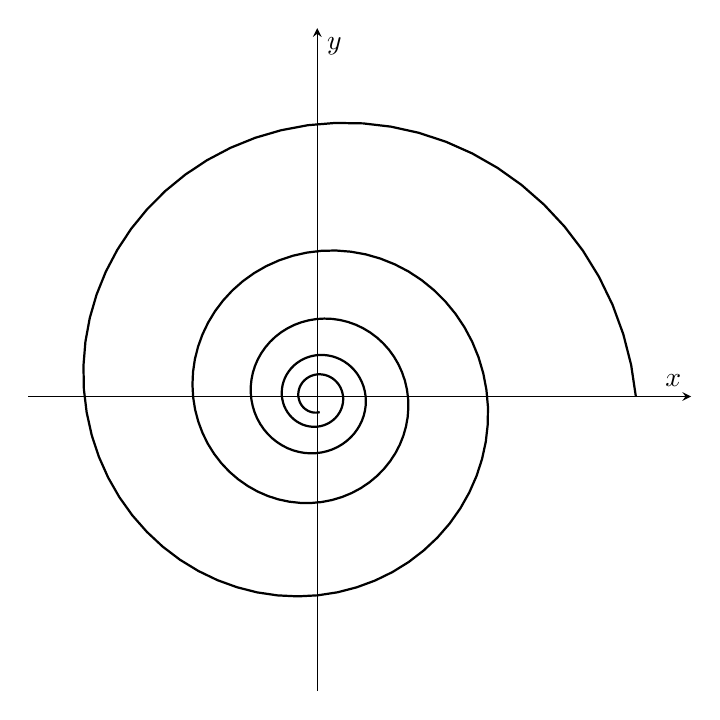
\begin{tikzpicture}
        \begin{axis}[
            axis lines = middle,    % Puts axes in the center
            axis equal,             % CRITICAL: Ensures the spiral isn't stretched/squished
            enlargelimits = true,   % Gives a little padding around the curve
            xlabel = {$x$},
            ylabel = {$y$},
            xtick = \empty,         % Removes numbers since it's a generic "sketch"
            ytick = \empty,
            width = 10cm,           % Adjust the size of your sketch here
            height = 10cm
        ]
        
        % The Logarithmic Spiral
        % We map t to 'x' in pgfplots. 
        % We use domain 0 to 30 radians (about 5 full rotations).
        % deg(x) converts the radians to degrees for the cos and sin functions.
        \addplot [
            domain=0:30, 
            samples=300,            % Higher samples = smoother curve
            thick, 
            black                   % You can change the color here
        ] 
        ( {1 * exp(-0.1 * x) * cos(deg(x))}, {1 * exp(-0.1 * x) * sin(deg(x))} );
        
        % Optional: Add a dot at the starting point (a, 0)
        % \addplot[mark=*, black] coordinates {(1,0)} node[above right] {$a$};

        \end{axis}
    \end{tikzpicture}
    \caption{Sketch of the curve $\gamma(t)$}
\end{figure}

\end{enumerate}

\newpage

\begin{problem}{Moment of inertia of an ellipsoid}{}
    \begin{enumerate}
        \item Determine the Jacobi determinant of the mapping
        \begin{align*}
            \Phi: \{ (s, t) : s \in (0, \infty),\ t \in (0, 2\pi) \} \rightarrow \R^2,\quad (s, t) \mapsto 
            \begin{pmatrix}
                as\cos t \\ bs\sin t   
            \end{pmatrix}
        \end{align*}

        in terms of the parameters $a, b > 0$.

        \item Calculate the polar moment of inertia
        \begin{align*}
            J_0 = \int_B x^2 + y^2 \dd \mathrm{vol}(x, y)
        \end{align*}

        of the ellipse $B = \{(x, y) \in \R^2 : \frac{x^2}{a^2} + \frac{y^2}{b^2} \leq 1\}$ with semi-axes $a, b > 0$.
    \end{enumerate}
\end{problem}

\begin{enumerate}
    \item The Jacobian of $\Phi$ is
    \begin{align*}
        J\Phi = 
        \begin{pmatrix}
            a\cos t & -a s \sin t \\
            b \sin t & b s \cos t
        \end{pmatrix}
    \end{align*}

    So, the determinant of the Jacobian is
    \begin{align*}
        \det(J\Phi) = abs\cos^2 t + abs \sin^2 t = abs
    \end{align*}

    \item We want to perform a change of variables using our parametrisation. Substitute $x = as\cos t,\ y = b s \sin t$
    \begin{align*}
        \frac{x^2}{a^2} + \frac{y^2}{b^2} = \frac{a^2s^2\cos^2 t}{a^2} + \frac{b^2s^2\sin^2 t}{b^2} = s^2 \cos^2 t + s^2 \sin^2 t = s^2 \leq 1
    \end{align*}

    So, we have $s \in (0, 1]$. Apply the change of variables to our integral:
    
    \begin{align*}
        J_0 &= \int_B x^2 + y^2 \dd \mathrm{vol}(x, y) 
        = 
        \int_{0}^{1} \int_{0}^{2\pi} \left(a^2s^2\cos^2 t + b^2s^2\sin^2 t\right) abs \dd t \dd s \\
        &= 
        \int_{0}^{1} \int_{0}^{2\pi} s^3 \left(a^3b\cos^2 t + ab^3\sin^2 t\right) \dd t \dd s \\
        &=
        \left(\int_{0}^{1} s^3 \dd s\right) \left(\int_{0}^{2\pi}  \left(a^3b\cos^2 t + ab^3\sin^2 t\right) \dd t\right) \\
        &= \left[\frac{1}{4}s^4\right]_0^1 
        \cdot 
        \left( a^3b \int_{0}^{2\pi} \cos^2 t \dd t + ab^3 \int_{0}^{2\pi}\sin^2 t \dd t \right) \\
        &= 
        \frac{1}{4} \left( a^3b \int_{0}^{2\pi} \frac{1 + \cos(2t)}{2} \dd t + ab^3 \int_{0}^{2\pi} \frac{1 - \cos(2t)}{2} \dd t \right) \\
    \end{align*}

    Let's solve these two integrals in the sum separately. The first is:
    \begin{align*}
        a^3b \int_{0}^{2\pi} \frac{1 + \cos(2t)}{2} \dd t &= \frac{1}{2}a^3b \int_{0}^{2\pi} \dd t + \frac{1}{2}a^3b \int_{0}^{2\pi} \cos(2t) \dd t \\
        &= a^3b\pi + \frac{a^3b}{4}\big[ \sin(2t) \big]_0^{2\pi} = a^3b\pi
    \end{align*}

    The second integral is:
    \begin{align*}
        ab^3 \int_{0}^{2\pi} \frac{1 - \cos(2t)}{2} \dd t &= \frac{1}{2}ab^3 \int_{0}^{2\pi} \dd t - \frac{1}{2}ab^3 \int_{0}^{2\pi} \cos(2t) \dd t \\
        &= ab^3\pi - \frac{ab^3}{4} \big[ \sin(2t) \big]_0^{2\pi} = ab^3\pi
    \end{align*}

    So the full integral is:
    \begin{align*}
        J_0 &= \frac{1}{4} \left( a^3b \int_{0}^{2\pi} \frac{1 + \cos(2t)}{2} \dd t + ab^3 \int_{0}^{2\pi} \frac{1 - \cos(2t)}{2} \dd t \right) \\
        &= \frac{1}{4} \left( a^3b\pi + ab^3\pi\right) = \boxed{\frac{ab\pi}{4} \left( a^2 + b^2 \right)}
    \end{align*}
\end{enumerate}

\end{document}